\chapter{State of the Art}
\lhead{\chaptername~\thechapter. \emph{State of the Art}}
\label{ch:state_of_the_art}
In this chapter we give a formal definition of the VO problem, we describe a 
general perspective SfM pipeline, then 
we explain the fundamental challenges issued by the employment of full 
spherical cameras for VO.
%
%
% Start of sections from intro
\section{Benefits of Full Spherical Cameras}
Because of the increased \textit{field of view} (FoV), panoramic cameras can capture a larger amount of data compared to traditional devices. For example, the two fisheye lenses in the Ricoh Theta allow users to utilize also rear correspondences between images and this may improve the quality of motion estimation.

Another advantage of full spherical cameras is that they do not require a calibration phase for intrinsic parameters estimation. Camera calibration is an essential requirement for most computer vision applications, which estimates several parameters such as focal length, image 
sensor size, pixel density, and lens distortion model. When dealing with full spherical cameras, we can assume the image is taken from a unitary sphere. Therefore, we can set the focal length to 1. Further details about the camera model and the parameters can be found in Chapter~\ref{ch:state_of_the_art}.

\section{SfM, VO, and SLAM}
SfM is a long studied topic in computer vision. Starting from an input of photographs taken by one or multiple cameras, SfM's main goal is to compute the cameras' poses and to reconstruct the 3D enviroment captured by those cameras.
%
Some of the first works are the paper by Longuet-Higgins\cite{longuet1981computer}, whose equations are fundamental in epipolar geometry, and the work by Tomasi et al.\cite{tomasi1992shape}, who used orthographic photographs to estimate the shape of a 3D object.
%
SfM is a general term, and it also includes \textit{visual odometry} (VO). This is the problem of recovering the motion of an agent equipped with a camera rig in a 3D environment. Typically, VO deals with an ordered set of images such as video sequences, and it uses them to compute the egomotion in real-time. Nister et al.\cite{nister2004visual} introduced the term \textit{visual odometry} for the first time.

Another field of robotic/computer vision research that is very close to VO is \textit{simultaneous localization and mapping} (SLAM). SLAM targets the problem of creating a map of the environment where a camera equipped agent navigates and simulatenously estimating its path. Scaramuzza\cite{scaramuzzaVisualOdometryI} pointed out that while VO is more focused on local motion estimation, SLAM's goal is to obtain a global consistent estimation of the agent movements.
%
In order to reduce error, SLAM keeps track of the visited path and can decide when the agent has come back to a previously visited location. This extra step in SLAM's pipeline is called \textit{loop closure} and provides an additional constraint used to reduce errors in both the agent's path and 
environment reconstruction. Durrant-White et al.\cite{durrant1996localization} firstly introduced the term SLAM.

%
% Francesco
%
 
\section{Densification: from Sparse to Dense Point Cloud}
A sparse point cloud is the product of most SfM pipelines; some key points are tracked in each photograph and are then used by the motion estimation algorithm. These key points are triangulated and their corresponding world points are available during egomotion estimation.
%
A set of triangulated key points is a sparse point cloud around the camera's path. This set provides a first approximation of the environment reconstruction.
Densification algorithms increase the number of matched points in two consecutive frames, this allows us to triangulate these points too. The result is a dense cloud of points around the camera's path that provides additional information about the surroundings' geometry or that can 
be the input data for surface reconstruction algorithms 
\cite{seitz2006comparison}.

In order to create a dense point cloud we need to produce the 
\textit{disparity map} from an image pair. This is a map of the distance in 
pixels from a point in a reference image and its corresponding point in the 
second image. The map is usually computed based on some kind of similarity 
metric such as \textit{sum of absolute distances} (SAD), 
\textit{sum of squared distances} (SSD), 
\textit{normalized cross correlation} (NCC), etc. These provides a way to 
compute the corresponding point in the second image, thus enabling the 
computation of the disparity for every point in the reference image.
Figure~\ref{fig:disparity_example} shows an example of disparity map.
\begin{figure}[h]
	\centering
	\begin{subfigure}{0.3\textwidth}
		\centering
		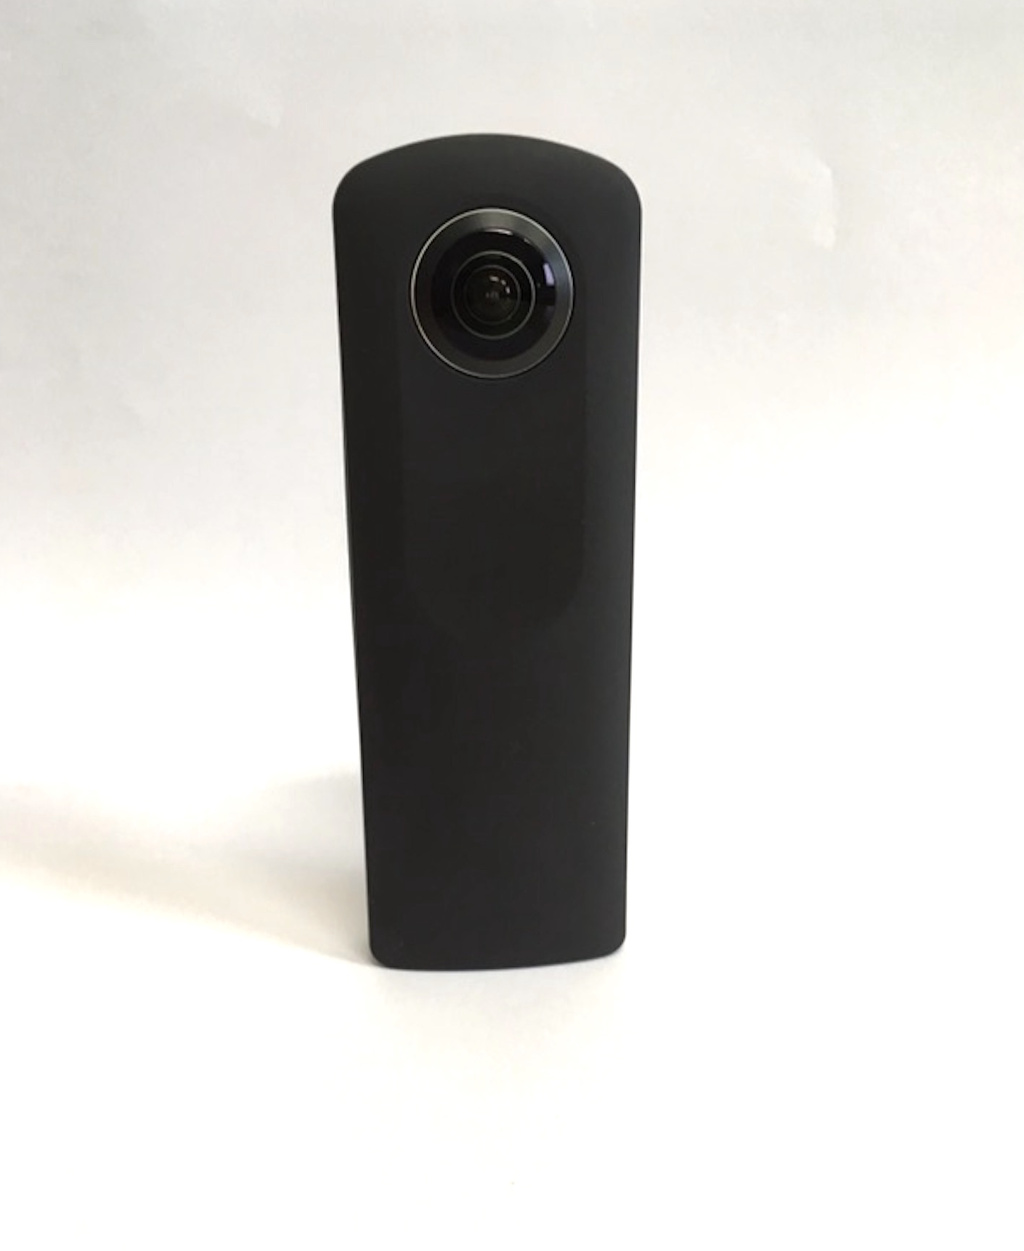
\includegraphics[width=0.7\textwidth]{img/theta1}
	\end{subfigure}
	\begin{subfigure}{0.3\textwidth}
		\centering
		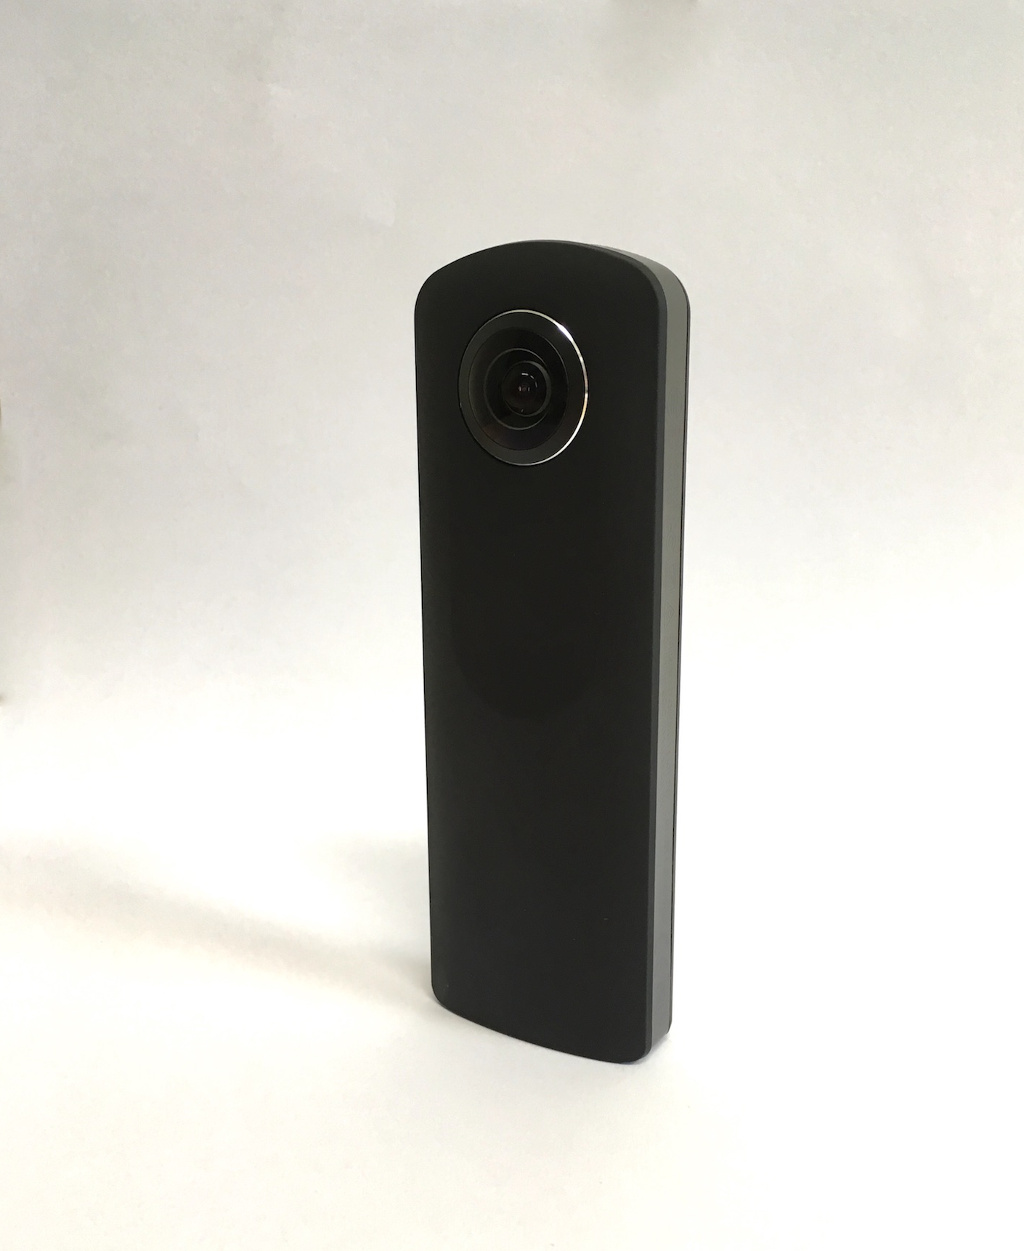
\includegraphics[width=0.7\textwidth]{img/theta2}
	\end{subfigure}
	\begin{subfigure}{0.3\textwidth}
		\centering
		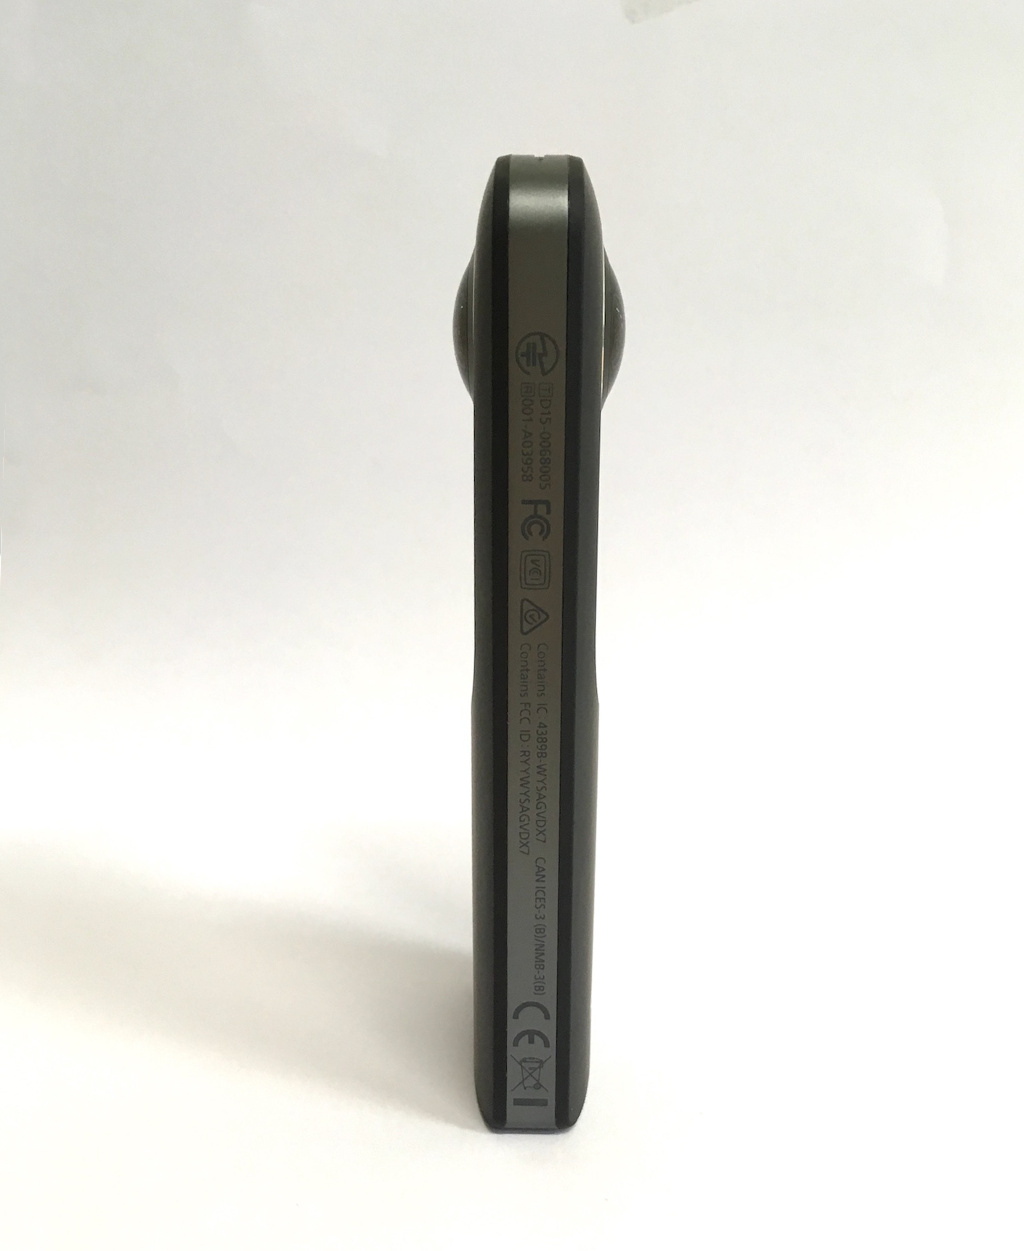
\includegraphics[width=0.7\textwidth]{img/theta3}
	\end{subfigure}
	\caption{\label{fig:disparity_example}The Ricoh Theta S 360\degree camera.}
\end{figure}
\todo[inline]{aggiungere disparity map example}

\section{Omnidirectional and Full Spherical Cameras}
\label{sec:cameraclassification}
Omnidirectional cameras are characterized by wide field of view. Indeed, many of this kind of devices can take pictures with a 180\degree view angle or even wider.

There are several ways to obtain panoramic images, they include:
\begin{itemize}
	\item perspective cameras and image stitching;
	\item catadioptric cameras;
	\item dioptric cameras;
	\item hybrid approaches.
\end{itemize}

Perspective cameras can take panoramic pictures with the aid of software stitching. As the first step, we take several photographs with many cameras or by simply moving the same camera in order to cover most of a scene. Then, a stitching software merges all images into a single one. To use a traditional camera and a stitching software is the cheapest way to obtain panoramic images because it does not need any kind of specialized hardware. However, this process is cumbersome (i.e., a lot of manual work for the user), and most importantly video sequences cannot be recorded. Note that some smart-phones provide built-in camera 360\degree acquisition modes, but the final quality may be not satisfactory due to alignment artifacts.
An example for this approach is the Hugin Panorama Photo Stitcher 
\cite{hugin_photostitcher}, an open source software for merging several 
perspective images in a single panoramic picture.
The SpheroCam\texttrademark by SPHERON-VR AG\texttrademark \cite{spheronvr}
is an alternative to 
the latter approach to panoramic images; it uses a specialized hardware composed
of a wide angle lenses equipped camera mounted on a rotating support. It can 
capture high quality full spherical and it addresses the professional fields of 
geographical analisys, forensic investigation, cultural heritage, etc.


Catadioptric cameras are obtained with a perspective camera and a mirror mounted in front of it. The camera take a picture of the mirror that reflects the surrounding. The mirror of a catadioptric system may have several shapes. The most common one is the hyperbolic profile that creates a single center of 
projection for every ray coming to the mirror.

A traditional camera can also be adapted to work as a panoramic one by adding a fisheye lens capable of refracting lights from wide angle towards the image sensor. These setups are called dioptric cameras.

Apart of perspective cameras coupled with stitching software, none of the previous approaches can take full spherical panoramic photographs. Moreover, full spherical videos cannot be shot with perspective cameras either.

The last approach, an hybrid one, exploits several sensors using fisheye lenses and software stitching to capture full spherical panoramic images in a single shot. This enables full spherical video capturing as well. The camera (that is composed of several image sensors) take multiple overlapping pictures simultaneously. Then, an on camera stitching software composes the data in a single image.

In all our experiments we used the Ricoh Theta S camera that is a hybrid full spherical camera 
composed of two fisheye lenses with a FOV greater than 180\degree; see Figure~\ref{fig:ricoh_theta}.
%
%
% end of sections from intro

\section{VO Problem}
\label{sec:vo_problem}
As we described in the previous chapter, the VO's goal is to recover the 
camera trajectory while it is moving in the environment. We now
introduce the notations we are going to use for the rest of this work; 
these are the same ones used by Scaramuzza in \cite{scaramuzzaVisualOdometryI}.
Let first assume time is sampled in a sequence of time instants \(k\); 
\(I_{0:n} \) is the set of input frames, with \(I_{k}\) the picture taken by 
the camera at time
\(k\). We define \(C_{0:n}\) as the set of camera 
positions such that \(C_k\) is the position at the \(k\)-th instant.
If we call \(T_k\) the rigid body transformation of the camera between the two
consecutive time instant $k-1$ and $k$, then we have the following relation:
\begin{equation}
	\label{eq:motion_composition}
C_n = C_{n-1} T_n
\end{equation}
\noindent with \(T_k\) defined as
\begin{equation*}
	T_k =
	\begin{bmatrix}
	R_k & \myvec{t}_k \\
	0 & 1
	\end{bmatrix} \text{.}
\end{equation*}
\noindent $R_k$ is a 3-by-3 rotation matrix while $\myvec{t}_k$ is a column vector, 
they represent the rotation and translation the camera performed from instant 
$k-1$ to $k$.
Therefore the goal of VO is to estimate both $R_k$ and $t_k$ for each instant 
$k$ and then compute the camera position $C_k$ accordingly to 
equation~\ref{eq:motion_composition}.
The initial position $C_0$ can be set arbitrarily.

Equation~\ref{eq:motion_composition} is the core of VO: thanks to it we are able
to compute the camera local movement, therefore we can estimate its location in 
every moment. But the equation above contains also the biggest practical 
challenge of VO, that is the error accumulation phenomenon known as 
\textit{drift}.
Every new position $C_k$ introduces an error factor that affects the next 
computations; the results is a global error that grows as the number of 
estimations increases.
All the efforts of the VO research community since early works like 
\cite{harris19883d} and \cite{moravec1980obstacle}, has focused on error
minimization techniques to reduce drift.
These tackle the precise estimation problem either by employing more accurate
local motion estimation and by introducing an optimization step to refine 
camera locations.
The set of techniques by which the drift is reduced once the camera poses have 
have been computed go under the general term \textit{bundle adjustment}.

\section{Perspective SfM}
The SfM literature is extensive but most of the approaches the 
researches followed so far present pipelines similar to the one in 
Fig.~\ref{fig:block_diagram}.
The main steps of the : compute the relative motion for each image
pair, then compose these motions to obtain the absolute camera position and 
orientation. Finally, run an optimization procedure to reduce drift.
The differences are in the type of input data, motion estimation algorithm,
optimization procedure and additional constraints considered.
For generic SfM researches, the input data is a set of traditional pictures of 
the same environment from different point of view. The pictures can be taken by 
different cameras with unknown parameters and in different time instants.
\begin{figure}
	\centering
	\def\svgwidth{0.5\columnwidth}
	\input{img/block_diagram.pdf_tex}
	\caption{Perspective SfM pipeline block diagram.}
	\label{fig:block_diagram}
\end{figure}
\textit{Visual Odometry} is based on SfM techniques, 
in this case, the input data is usually a sequence 
of images from a video stream. Many studies targeted different hardware setup 
but the specific image capturing device is usually either a single perspective 
camera or a stereo imaging rig. The computer vision literature refers to the
former case with the term \textit{monocular VO} while it uses \textit{stereo VO}
to describe the latter.

Even though perspective cameras have been the first choice in many studies, 
the researchers used other devices, like the ones described in 
\ref{sec:cameraclassification}.

We use the terms \textit{perspective} or \textit{traditional SfM} to describe 
SfM pipelines designed for perspective cameras.

A great resource about the state of the art for Visual Odometry and Structure 
from Motion techniques is the couple of articles by Scaramuzza,  
\cite{scaramuzzaVisualOdometryI} and \cite{scaramuzzaVisualOdometryII}.

\subsection{Motion Estimation}
\label{subsec:motion_estimation}
We use the term local motion to indicate the camera movement between two 
consecutive images while, on the other hand, we define global motion as
the overall camera's path.
The local motion estimation step is fundamental in a SfM pipeline, its goal is 
to find the rigid body transformation composed of $R_k$ and $t_k$ as we 
described in Section~\ref{sec:vo_problem}.
All the local motion estimation methods described in the literature so far are 
based on the correspondences found in two consecutive images but, depending on the
specific camera rig (stereo imaging systems or monocular), the type of 
correspondences and their matching procedure, we may have several choices for
the actual way to estimate local motion.
There are two main families of point matching algorithms: \textit{feature-based}
and \textit{appearance-based} (also known as \textit{global-methods}).
While the former ones utilize repeatable features 
matching between the images, the latter rely on pixel's intensity information; 
they are simpler but also slower. Most of the 
most recent VO pipelines use feature-based methods because of
their speed and robustness.
A VO implementation that employs intensity based techniques is 
\cite{nister2004visual}, while \cite{makadia2007correspondence} is an example 
of featureless motion estimation method.

Each of the feature points found by the motion estimation phase can be 
either a 3D world-point feature or a 2D image-point one,
therefore, there are three possible combinations that provides just as many 
different matching and motion-estimation procedures:
\begin{itemize}
	\item 2D-to-2D: both feature sets are composed of image points.
The matching metric can be a simple euclidean distance between feature 
descriptors and the motion estimation can be solved by estimating the 
\textit{essential matrix} (see section~\ref{subsec:essential_matrix} for 
details);
	\item 3D-to-3D: both feature sets contain world-points features and motion
estimation is performed by solving an alignment problem;
	\item 3D-to-2D: the previous image's feature set is composed of world points while
the current one's feature set contains their projections. In this case, the motion 
is estimated by solving a \textit{PnP} problem.
\end{itemize}
Since the second and third approaches deal with 3D points, they are usually 
best suited for stereo rig (especially the 3D-to-3D case).
Yet we can still use the 3D-to-2D approach in the monocular VO case by simply 
triangulating corresponding 2D image features in consecutive frames.
In fact, in order to obtain the first 3D feature set,
we can compute the relative motion between the first two images with 
the 2D-to-2D techniques and then obtain the rest of the camera's path,
as we said, by solving the \textit{PnP} problem.

\subsubsection{Essential Matrix}
\label{subsec:essential_matrix}
The essential matrix $E$ is defined by the equation
\begin{equation}
\label{eq:epipolar_equation}
\mathbf{p}'^\top E \mathbf{p} = 0
\end{equation}
\noindent where $\mathbf{p}$ and $\mathbf{p}'$ are the normalized corresponding 
feature coordinates in the image $I_{k-1}$ and $I_{k}$ respectively.
The normalized coordinates are defined as:
\begin{equation}
	\mathbf{p} = K^{-1} \mathbf{m}
\end{equation}
\noindent where $K$ is the intrinsic parameter matrix and $\mathbf{m}$ is an
image point.
The essential matrix contains the geometric information that describe the 
relative location of a camera respect to another one up to an unknown scale factor 
for the translation vector. In particular, we have
\begin{equation*}
	E_k = \lambda \hat{t}_kR_k
\end{equation*}
\noindent with $\lambda$ that is the unknown scale factor and $\hat{t}_k$ is 
the skew-symmetric form for the cross product of vector $t_k$.
In order to extract the local motion given the two set of corresponding features
in two consecutive images, we have to estimate the essential matrix and then 
extract the rigid body transformation out of it.
For the $E$ estimation part we can employ the Longuet-Higgins' 8-points 
algorithm \cite{longuet1981computer}: the equation~\ref{eq:epipolar_equation} 
provides a constraint we
can exploit for computation, in fact, for each correspondence, we can rewrite 
the equation as
\begin{equation*}
	\begin{bmatrix}
		p_1p'_1 & p'_1p_2 & p'_1 & p_1p'_2 & p_2p'_2 & p'_2 & p_1 & p_2 & 1
	\end{bmatrix}
	E = 0	\text{.}
\end{equation*}
To find the nine unknowns we need 8 noncoplanar feature matches that provide as many 
independent equations.
In practice we use more than 8 points, therefore we obtain a overdetermined 
system we solve in the least square sense.

Once $E$ has been estimated, there are 4 possible combinations for the relative 
position of the two cameras and each world points. We are interested in the one
that presents both cameras facing toward the triangulated world point,
i.e. this point has to be in front of both cameras. We can easily chose the 
correct configuration among the four by testing each of them.

\subsubsection{Relative Scale}
As we have already pointed out in the previous section, every monocular SfM 
pipeline that works with 2D-to-2D feature correspondences can estimate the 
local motion up to an unknown scale factor. In fact, there is no way to extract 
the translation magnitude from two sets of features (it is still possible 
to recover the reconstruction scale if we are given some world measure of the
environment).
Therefore, if we can not derive the local translation length with some other
non visual techniques (like wheel odometry, GPS, accelerometer, etc.), 
all we can do is to leave the unknown scale for the motion estimation and 
environment reconstruction.

On the other hand, if we have to compose the motion of more than two poses, 
like VO does, we need to set the first local translation magnitude 
arbitrarily and express all the other movements relative to this first one.
This means that we need to compute the \textit{relative scale}
for every translation other than the first one.

A possible approach for relative scale estimation is described in 
\cite{scaramuzzaVisualOdometryI}. If we want to estimate the relative scale for 
the motion $t_k$, between instants $k-1$ and $k$, we need to compute the 
two sets of triangulated world points $X_{k-1}$ and $X_{k}$ by using 
the two image pairs $I_{k-2}$ and $I_{k-1}$ , and  $I_{k-1}$ and  $I_{k}$ first; then,
given $i$ and $j$, two world points that belongs to both sets $X_{k-1}$ and 
$X_{k}$, we can compute the relative scale accordingly to these points with
\begin{equation}
	\label{eq:relative_scale}
	r = \frac{\| X_{k-1, i} - X_{k - 1, j} \|}{\| X_{k, i} - X_{k, j} \|}
	\text{.}
\end{equation}
\noindent For each world points pair, we obtain a different values of $r$;
we can then select the average of $r$ (or better, its median in case of 
outliers).

It is worth noticing that the exact \textit{absolute scale} for the whole 
camera motion and environment reconstruction is still left unknown.
\todo{aggiungere citazioni}

\section{Bundle Adjustment}
We have already introduced the error accumulation problem that affects SfM in 
section~\ref{sec:vo_problem}; because of the unavoidable errors we introduce 
for each camera pose estimation, an SfM pipeline incorporates a 
refinement process for both camera poses and triangulated points.
This step is called \textit{bundle adjustment} (BA) and its goal is to 
minimize the \textit{reprojection error}.
Point reprojection is the function that projects a world point to image space; 
in particular, the reprojection ${\myvec{\bar{m}}_i}^j$ of the scene point 
$\myvec{M}^j$ according to camera $i$ is defined as
\begin{equation*}
	{\myvec{\bar{m}}_i}^j = K_i[R_i | \myvec{t}_i]\myvec{M}^j	\text{.}
\end{equation*}
\noindent Bundle adjustment can then be expressed as the following minimization 
problem
\begin{equation*}
	\label{eq:bundle_adj}
	\min_{R_i, \myvec{t}_i, \myvec{M}^j} 
	\sum_{i = 1}^N\sum_{j = 1}^n 
	d(K_i[R_i | \myvec{t}_i]\myvec{M}^j, \myvec{m}_i^j) \text{,}
\end{equation*}
\noindent with $\myvec{m}_i^j$ that is the image point of the $i$-th camera
corresponding to $\myvec{M}^j$.
This non linear least squares minimization is usually solved with the 
Levenberg–Marquardt method 
\cite{triggs1999bundle,Hartley2004,levenberg1944method}.
The term \textit{bundle} refers to the fact that both the camera position and
the triangulated points are jointly refined. Most BA implementations keep the 
camera poses fixed, solve for the triangulated points and then optimize for the
poses in an alternate fashion until the desired precision is reached.

BA is a delicate step that can affect an SfM pipeline in many ways
\cite{lourakis2009sba,triggs1999bundle,Hartley2004} as a poorly planned use of 
it can reduce computation speed and fail to obtain the desired accuracy.

\section{Robust Estimation}
In the previous sections, we described the core steps of an SfM pipeline.
Even though these are all the components needed for a working SfM software, 
there are some improvements widely used by similar pipelines nowadays
that can further increase the reconstruction and pose estimation 
precision and robustness, and, in general, make these pipelines more effective.
In the following sections we review some of the most common improvements 
employed in SfM software.

\begin{figure}
	\centering
	\begin{subfigure}{\textwidth}
		\centering
		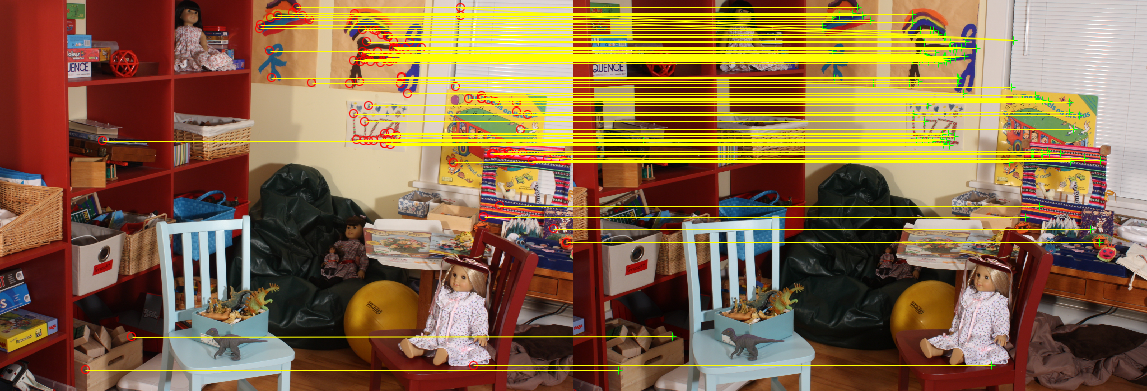
\includegraphics[width=\textwidth]{img/good_stereo}
		\caption{A subset of the matches found in this image pair.}\label{fig:good_stereo}
	\end{subfigure}
	\begin{subfigure}{\textwidth}
		\centering
		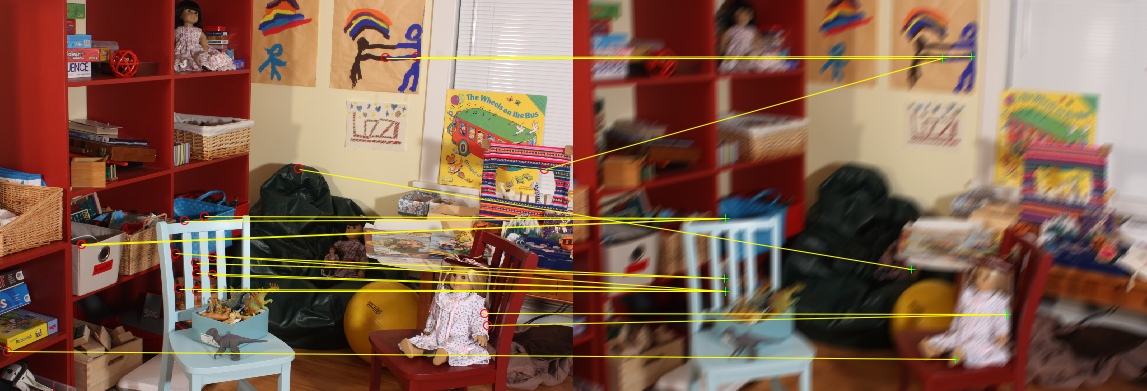
\includegraphics[width=\textwidth]{img/motion_blur}
		\caption{Motion blur reduce both the number and quality of matches.}\label{fig:motion_blur}
	\end{subfigure}
	\begin{subfigure}{\textwidth}
		\centering
		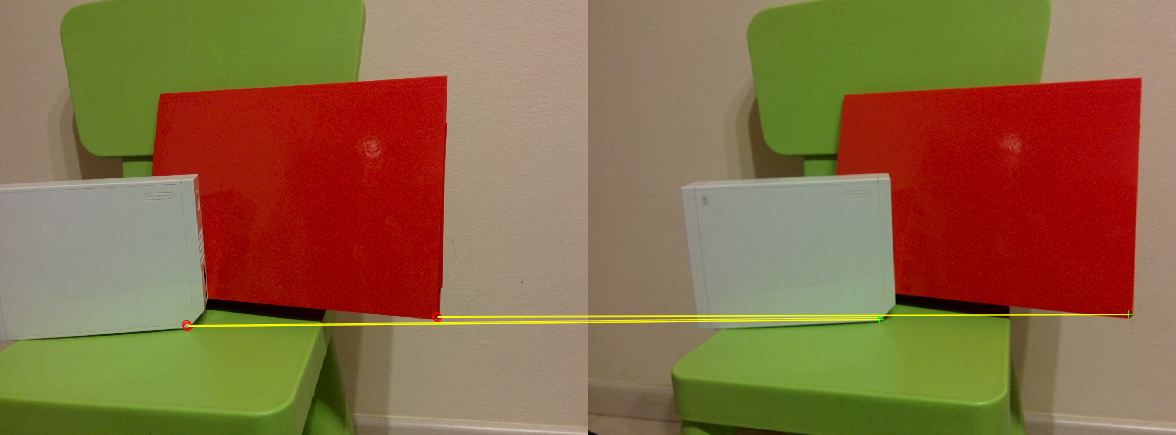
\includegraphics[width=\textwidth]{img/textureless_stereo}
		\caption{Textureless images provides too less feature points.}\label{fig:textureless}
	\end{subfigure}
	\caption{Some examples of problems that may occur during correspondence search.}\label{fig:matching_problems}
\end{figure}

\subsection{Feature Detectors}
As we discussed in section~\ref{subsec:motion_estimation}, in order to estimate
the essential matrix, we need to find corresponding points in image pairs; 
these points are \textit{feature points} (or \textit{interesting points}).
Feature points are patterns in images that are likely to be unique; 
a feature point is usually described by a vector called 
\textit{feature descriptor}.
There are many different types of feature and descriptors like 
\textit{Moravec detector} \cite{moravec1980obstacle}, \textit{Harris
corner detector} \cite{harris1988combined}, 
\textit{SIFT} \cite{lowe1999object}, etc.
Some of this features are affected by rotations and scale; since SfM is based on
many pictures taken from different views, SIFT features have always been 
preferred over other less robust features because of their rotational and scale
invariance. One of the main drawback is that 
SIFT is patented and can note be used freely as other detectors.
SURF \cite{funayama2012robust} is another kind of features that, 
just like SIFT, is rotational and scale invariant but whose implementation is 
available within the main computer vision framework because of lesser 
restrictions.
For a more detailed discussion about the differences among point detectors, 
see \cite{schmidt2010evaluation,govender2009evaluation}.

\subsection{Outliers Rejection}
Since the motion estimation step is the core of SfM pipelines, its performance
affects the overall software; in particular, motion estimation is influenced 
by the presence of outliers in features matching.
A matching outlier is a pair of feature points that are erroneously considered 
corresponding points. If the motion estimation phase considered these points for
its computation, the result would be unreliable and it could compromise the 
whole camera's path estimation because of the incremental nature of the SfM 
pipeline.
In order to reduce this phenomenon, we can switch to a more robust feature 
detector and add the famous RANSAC algorithm to remove outliers before the 
motion estimation step.
RANSAC \cite{fischler1981random} is a model fitting algorithm for dataset 
that includes outliers.
It is an iterative process that selects a subset of 
input data at every iteration and computes the model based on this subset only;
it then divides the complete dataset into a consensus set and outliers, if
the number of outliers, computed thanks to a problem specific loss function, is
less than a given threshold, the estimated model is considered valid.

RANSAC is now a standard step in SfM. It selects the correspondences inliers at
random, computes the essential matrix accordingly to the selected matches and
evaluates the outliers based on the reprojection error defined as:
\begin{equation*}
	Err =  
	\sum_{i = 1}^N\sum_{j = 1}^n 
	d(K_iE\myvec{M}^j, \myvec{m}_i^j) \text{.}
\end{equation*}
This error formulation is similar to equation~\ref{eq:bundle_adj} but now the
essential matrix is not decomposed in $[R_i|\myvec{t}_i]$.
The use of RANSAC before motion estimation provides a more reliable result if
the number of outliers is not prevalent.

\section{Full Spherical Cameras}
\subsection{Image Format}
If we consider the simplest camera model, 
a perspective image is the result of the intersection between the image plane 
and all the light rays that go from the environment to the center of 
projection inside the camera (see Fig\ref{fig:perscam_model}).
\missingfigure{aggiungere modello camera prospettica}
\label{fig:perscam_model}
On the other hand, the full spherical camera model implies the image plane 
to be the result of the intersection between a sphere and the rays from the 
environment to the center of projection (which is equivalent to the sphere's 
center).

